%%% If you use this template then please give credit like this:
%%% ----------------------------
% LaTeX code inspired by the LaTeX Thesis Template by Manuel Kuehner
% www.bedienhaptik.de/latex-template/
%%% ----------------------------

%\overfullrule=2cm


%\newcommand{\finalversion}{}    
\documentclass%
[%
paper=a4
,fontsize=12pt % common are 10, 11 or 12
,headings=big
,cleardoublepage=current
,numbers=noendperiod % 2.3.1 vs 2.3.1. (no dot after the last chapter number)
,twoside=true
,toc=bibliography % Bibliography appears in Table of Contents (without a number)
,toc=listof % List of Figures and List of Tables appear in Table of Contents
,version=last % Use latest version of the KOMA-Script
]%
{scrbook}

%\renewcommand*{\familydefault}{\sfdefault}
%  \def\tt{\normalfont\ttfamily}

\ifx\finalversion\undefined
\overfullrule=2cm
\fi

%%% Local Variables:
%%% mode: latex
%%% TeX-master: "../main"
%%% End:


% Standard packages
%%% File encoding is ISO-8859-1 (also known as Latin-1)

% Input encoding is 'latin1' (Latin 1 - also known as ISO-8859-1)
% CTAN: http://www.ctan.org/pkg/inputenc
%
% A newer package is available - you may look into:
% \usepackage[x-iso-8859-1]{inputenc}
% CTAN: http://www.ctan.org/pkg/inputenx
\usepackage[utf8]{inputenc}

% CTAN: http://www.ctan.org/pkg/fontenc
\usepackage[T1]{fontenc}

% Language support for 'english' (alternative 'ngerman' or 'french' for example)
% CTAN: http://www.ctan.org/pkg/babel
\usepackage[english]{babel}

% Doing calculations with LaTeX units -- needed for the vertical line in the footer
% CTAN: http://www.ctan.org/pkg/calc
\usepackage{calc}
\usepackage[nomessages]{fp}% http://ctan.org/pkg/fp

% Proper units in math mode
\usepackage{siunitx}

% Extended graphics support
% There is also a package named 'graphics' - watch out!
% CTAN: http://www.ctan.org/pkg/graphicx
\usepackage{graphicx}
\usepackage{varwidth}

% Extendes support for floating objects (tables, figures), adds the [H] placing option (\begin{figure}[H]) which palces it "Here" (without any doubt).
% CTAN: http://www.ctan.org/pkg/float
\usepackage{float}

% Extended color support
% I use the command \definecolor for example.
% Option 'Table': Load the colortbl package, in order to use the tools for coloring rows, columns, and cells within tables.
% CTAN: http://www.ctan.org/pkg/xcolor
\usepackage[table,svgnames]{xcolor}

% Nice tables
% CTAN: http://www.ctan.org/pkg/booktabs
\usepackage{booktabs}

% Better support for ragged left and right. Provides the commands \RaggedRight and \RaggedLeft.
% Standard LaTeX commands are \raggedright and \raggedleft
% http://www.ctan.org/pkg/ragged2e
\usepackage{ragged2e}

%\usepackage{cleveref}

% Create function plots directly in LaTeX
% CTAN: http://www.ctan.org/pkg/pgfplots

%%%%%%%% Packages %%%%%%%%%%%
\usepackage[printonlyused]{acronym}

%\renewcommand*{\acsfont}[1]{\textcolor{red}{#1}} 
%\renewcommand*{\acffont}[1]{\textbf{{#1}}}

\usepackage{appendix}
\usepackage{pgfgantt}

%\usepackage{acro}
\usepackage{epigraph}

\usepackage{needspace}

\usepackage{amsmath}
\usepackage{upgreek}
\usepackage{xfrac}
\usepackage{mhchem}
\usepackage{gensymb}%For \degree

\usepackage{blindtext}
\usepackage{comment}
\usepackage{graphicx}
\usepackage{helvet}
\usepackage{times}

\usepackage{listings}
\lstset{
  language=python,
  literate=%
    {0}{{{\color{lime!50!black}0}}}1
    {1}{{{\color{lime!50!black}1}}}1
    {2}{{{\color{lime!50!black}2}}}1
    {3}{{{\color{lime!50!black}3}}}1
    {4}{{{\color{lime!50!black}4}}}1
    {5}{{{\color{lime!50!black}5}}}1
    {6}{{{\color{lime!50!black}6}}}1
    {7}{{{\color{lime!50!black}7}}}1
    {8}{{{\color{lime!50!black}8}}}1
    {9}{{{\color{lime!50!black}9}}}1,
  basicstyle=\sffamily,
  keywordstyle=\sffamily\bfseries\color{orange!60!black},
  identifierstyle=\color{teal!40!black},
}

\usepackage{makeidx}
\usepackage{multirow}

\usepackage{url}

\usepackage{hologo}

\usepackage{float}
\usepackage{caption}
\usepackage{subcaption}
\usepackage[export]{adjustbox}

\usepackage{etoolbox}
\usepackage{pgfgantt}
\usepackage{rotating}
\usepackage{relsize}

\providecommand{\description}{}
\usepackage{paralist}
\usepackage{enumerate}
\usepackage{enumitem}

\makeatletter
\@ifundefined{previewmode}{}{
\usepackage[tightpage,active,noconfig]{preview}
}
\makeatother

\usepackage[normalem]{ulem}

\ifx\finalversion\undefined
\usepackage[color=green!40, colorinlistoftodos, figwidth=\columnwidth]{todonotes}
\newcommand{\todoI}[1]{

\resizebox{0.95\columnwidth}{!}{\todo[inline]{#1}}}
\else
\newcommand{\todoI}[1]{}
\newcommand{\todo}[1]{}
\newcommand{\listoftodos}{}
\fi



%%% Local Variables:
%%% mode: latex
%%% TeX-master: "../main"
%%% End:


\ifx\darkmode\undefined
\definecolor[named]{myColorMainA}{RGB}{0,0,0}
\definecolor[named]{myColorMainB}{RGB}{174,49,54}
\else
\definecolor[named]{myColorMainA}{RGB}{223,223,223}
\definecolor[named]{myColorMainB}{RGB}{174,49,54}
\fi

% Math related
\usepackage{amsfonts}
\usepackage{amsmath}
\usepackage{amsmath, amsthm, amssymb}
\usepackage{amsthm}

\newtheorem{definition}{Definition}
\newtheorem{theorem}{Theorem}[section]
\newtheorem{lemma}{Lemma}[section]
\newtheorem{proposition}{Proposition}[section]
\newtheorem{corollary}{Corollary}[section]
\renewcommand{\qedsymbol}{\rule{0.7em}{0.7em}}


% Algorithm
\usepackage[chapter]{algorithm}
\usepackage{algcompatible}
\usepackage{algorithmicx}
\usepackage{algpseudocode}
\usepackage{eqparbox}
\usepackage{xpatch}
% Line separation
\makeatletter
\xpatchcmd{\algorithmic}{\itemsep\z@}{\baselineskip=1.1em}{}{}
\makeatother

\algrenewcommand\alglinenumber[1]{\footnotesize #1}%

\renewcommand{\algorithmiccomment}[1]{\hfill\eqparbox{COMMENT}{\# #1}}

\makeatletter
\providecommand\theHALG@line{\thealgorithm.\arabic{ALG@line}}
\makeatother


\makeatletter
% code borrowed from Andrew Stacey; See
% http://tex.stackexchange.com/a/50054/3954
\tikzset{%
    remember picture with id/.style={%
        remember picture,
        overlay,
        save picture id=#1,
    },
    save picture id/.code={%
        \edef\pgf@temp{#1}%
        \immediate\write\pgfutil@auxout{%
            \noexpand\savepointas{\pgf@temp}{\pgfpictureid}}%
    },
    if picture id/.code args={#1#2#3}{%
        \@ifundefined{save@pt@#1}{%
            \pgfkeysalso{#3}%
            }{
            \pgfkeysalso{#2}%
        }
    }
}

\def\savepointas#1#2{%
    \expandafter\gdef\csname save@pt@#1\endcsname{#2}%
}

\def\tmk@labeldef#1,#2\@nil{%
    \def\tmk@label{#1}%
    \def\tmk@def{#2}%
}

\tikzdeclarecoordinatesystem{pic}{%
    \pgfutil@in@,{#1}%
    \ifpgfutil@in@%
    \tmk@labeldef#1\@nil
    \else
    \tmk@labeldef#1,(0pt,0pt)\@nil
    \fi
    \@ifundefined{save@pt@\tmk@label}{%
        \tikz@scan@one@point\pgfutil@firstofone\tmk@def
        }{%
        \pgfsys@getposition{\csname save@pt@\tmk@label\endcsname}\save@orig@pic%
        \pgfsys@getposition{\pgfpictureid}\save@this@pic%
        \pgf@process{\pgfpointorigin\save@this@pic}%
        \pgf@xa=\pgf@x
        \pgf@ya=\pgf@y
        \pgf@process{\pgfpointorigin\save@orig@pic}%
        \advance\pgf@x by -\pgf@xa
        \advance\pgf@y by -\pgf@ya
    }%
}

% end of Andrew's code

\newlength\AlgIndent
\setlength\AlgIndent{0pt}
% main command to draw the colored background
\newcounter{mymark}
\newcommand\ColorLine{%
  \stepcounter{mymark}%
  \tikz[remember picture with id=mark-\themymark,overlay] {;}%
  \begin{tikzpicture}[remember picture,overlay]%
    \filldraw[lime!70!black,fill opacity=0.5,draw=none]%teal!40!white]%
    let \p1=(pic cs:mark-\themymark),
    \p2=(current page.east)  in
    ([xshift=-\ALG@thistlm-0.3em,yshift=-0.5em]0,\y1)  rectangle ++(\linewidth+\AlgIndent,\baselineskip+0.41em);
  \end{tikzpicture}%
}%

\algnewcommand\CSTATE{\State\ColorLine}%

 \algdef{SE}[IF]{CIF}{ENDIF}%
 [2][default]{\ColorLine\algorithmicif\ #2\ \algorithmicthen\ALG@compatcomm{#1}}%
 {\algorithmicend\ \algorithmicif}%

\makeatother
\algtext*{EndFor}% Remove "end while" text
\algtext*{EndWhile}% Remove "end while" text
\algtext*{EndIf}% Remove "end if" text


% PDF related packages
%%% File encoding is ISO-8859-1 (also known as Latin-1)
%%% You can use special characters just like �,� and �

% Package for PDF features such as bookmarks and hyperlinks.
% Important: Should be loaded at the end.
% CTAN: http://www.ctan.org/pkg/hyperref
\definecolor{hyperrefcolor}{gray}{0}

\usepackage[%
bookmarks, % Create bookmarks
bookmarksopen=true, % Unfold bookmatk tree in PDF viewer when document is opened
bookmarksopenlevel=1, % Level of unfolding
bookmarksnumbered=true, % Number bookmarks
hidelinks, % do not highlight hyperlinks -- looks ugly
% Ansicht beim �ffnen
pdfpagelabels=true, % See manual...
plainpages=false, % See manual...
hyperfootnotes=true, % Hyperlinks for footnotes
hyperindex=true, % Indexeintr�age verweisen auf Text
colorlinks=true,
linkcolor=hyperrefcolor,
citecolor=hyperrefcolor,
urlcolor=hyperrefcolor,
hypertexnames=true,
pagebackref=true]{hyperref}

%%% Local Variables:
%%% mode: latex
%%% TeX-master: "../main"
%%% End:


% Bibliography related
\DeclareRobustCommand{\van}[3]{#2 #1}

\usepackage[square,sort,comma]{natbib}
%\bibliographystyle{abbrvnat}
\bibliographystyle{apalike}

%

\setcitestyle{square}


\newlength\mybibindent
\setlength\mybibindent{10mm}

\makeatletter

\renewenvironment{thebibliography}[1]
     {\chapter*{\bibname}%
      \@mkboth{\bibname}{\bibname}%
      \addcontentsline{toc}{chapter}{\bibname}

      \list{\@biblabel{\@arabic\c@enumiv}}%
           {\settowidth\labelwidth{\@biblabel{#1}}%
            \leftmargin\labelwidth
            \advance\leftmargin\dimexpr\labelsep+\mybibindent\relax\itemindent-\mybibindent% new
            \@openbib@code
            \usecounter{enumiv}%
            \let\p@enumiv\@empty
            \renewcommand\theenumiv{\@arabic\c@enumiv}}%
      \sloppy
      \clubpenalty4000
      \@clubpenalty \clubpenalty
      \widowpenalty4000%
      \sfcode`\.\@m}
     {\def\@noitemerr
       {\@latex@warning{Empty `thebibliography' environment}}%
      \endlist}
\def\@lbibitem[#1]#2{%
\if\relax\@extra@b@citeb\relax\else
\@ifundefined{br@#2\@extra@b@citeb}{}{%
\@namedef{br@#2}{\@nameuse{br@#2\@extra@b@citeb}}}\fi
\@ifundefined{b@#2\@extra@b@citeb}{\def\NAT@num{}}{\NAT@parse{#2}}%
\item[\hfil\hyper@natanchorstart{#2\@extra@b@citeb}{\protect\NoHyper\citep{#2}\protect\endNoHyper}%
\hyper@natanchorend]%
\NAT@ifcmd#1(@)(@)\@nil{#2}}
\makeatother


% nicer backref links
\renewcommand*{\backref}[1]{}
\renewcommand*{\backrefalt}[4]{%
\ifcase #1 %
%(Not cited.)%
\relax
\or
(Cited on page~#2)%
\else
(Cited on pages~#2)%
\fi}
\renewcommand*{\backrefsep}{, }
\renewcommand*{\backreftwosep}{ and~}
\renewcommand*{\backreflastsep}{ and~}


% PDF related packages
%%% File encoding is ISO-8859-1 (also known as Latin-1)
%%% You can use special characters just like �,� and �

% Package to create test text -- just for demonstration purposes
% The command \blindtext produces a test text -- good for testing the layout
% CTAN: http://www.ctan.org/pkg/blindtext
\usepackage[]{blindtext}
% The custom command \myMarginnote is defined in the file:
% 01_Preamble/HeaderFooterMarginnote.tex
\renewcommand{\blindmarkup}[1]{#1}


% Custom Macros
\usepackage{bm}

\DeclareMathOperator*{\argmax}{arg\,max}
\newcommand{\imply}{\Rightarrow}
\newcommand{\diag}{\mathit{D}}
\newcommand{\COMPS}{\mathit{COMPS}}
\newcommand{\SD}{\mathit{SD}}
\newcommand{\DS}{\mathit{DS}}
\newcommand{\OBS}{\mathit{OBS}}
\newcommand{\OBSJ}{\OBS_j}


\providecommand{\e}[1]{\ensuremath{\times 10^{#1}}}
\newcommand{\fn}[1]{\bm{\mathit{#1}}}
\newcommand{\set}[1]{\{#1\}}
\newcommand{\angledlist}[1]{\langle #1 \rangle}

\newcommand{\pr}[1]{\fn{Pr}(#1)}
\newcommand{\likelihoodii}[2][d]{\pr{A_{#2},e_{#2}\mid #1}}
\newcommand{\likelihoodi}[1][d]{\pr{A_i,e_i\mid #1}}
\newcommand{\likelihood}[1][d]{\pr{A,e\mid #1}}
\newcommand{\prior}[1][d]{\pr{#1}}
\newcommand{\posterior}[1][d]{\pr{#1\mid A,e}}
\newcommand{\gFunc}[1][d]{\fn{G}(#1, A_i)}

\newcommand{\likelihoodcii}[2][d]{\pr{A_{#2},e_{#2},c_{#2}\mid #1}}
\newcommand{\likelihoodci}[1][d]{\pr{A_i,e_i,c_i\mid #1}}
\newcommand{\likelihoodc}[1][d]{\pr{A,e,c\mid #1}}
\newcommand{\posteriorc}[1][d]{\pr{#1\mid A,e,c}}

\newcommand{\nfunc}[1]{\fn{n}_{#1}(j)}

\newcommand{\mTrue}{\mathit{True}}
\newcommand{\mFalse}{\mathit{False}}


%Staccato
\newcommand{\bigO}[1]{\fn{\mathcal O}\big(#1\big)}
\newcommand{\powSet}[1]{\fn{\mathcal P}(#1)}

\newcommand{\staccato}{\textit{Staccato}}
\newcommand{\mhsII}{\texorpdfstring{$\textit{MHS}^\text{\smaller2}$}{MHS2}}
\newcommand{\mhsIIURL}{\url{https://github.com/npcardoso/MHS2}}

\newcommand{\HS}{\fn{HS}}
\newcommand{\MHS}{\fn{MHS}}

\newcommand{\setupName}[1]{\textit{#1}}
\newcommand{\Opt}[1]{\setupName{Opt $\mathit{#1}$}}
\newcommand{\Opts}[2]{\setupName{Opts $\mathit{#1}$ -- $\mathit{#2}$}}


% Fuzzinel
\newcommand{\cerror}[1][F]{\fn{\mu_{#1}}}
\newcommand{\ferror}[1][F]{\fn{\mu_{\widetilde{#1}}}}
\newcommand{\fuzzinel}{\texorpdfstring{$\textit{Fuzzinel}$}{Fuzzinel}}

% NFGE
\newcommand{\BW}{\mathit{bw}}
\newcommand{\ST}{\mathit{st}}
\newcommand{\FB}{\mathit{Fb}}
\newcommand{\KDEfunc}[1][ej]{\fn{\hat{f}_{#1}}}
\newcommand{\KDE}[1][ej]{\KDEfunc[#1](\ST)}
\newcommand{\NFGE}{\texorpdfstring{$\textit{NFGE}$}{NFGE}}
\newcommand{\supergjcomb}[1][j]{\fn{g^+_{#1}}(\ST)}
\newcommand{\supergjcall}[2][\ST]{\texorpdfstring{\fn{\breve{g}_{#2}}(#1)}{g#2(#1)}}
\newcommand{\supergj}[1][j]{\supergjcall{#1}}


\newcommand{\supergFunc}[1][j,S]{\fn{\breve{G}}(#1)}

\newcommand{\etc}{\emph{etc.}}
\newcommand{\ie}{\emph{i.e.}}
\newcommand{\eg}{\emph{e.g.}}
\newcommand{\vs}{\textit{vs.}}


\newcommand{\CrefPageParen}[1]{\Cref{#1} (page \pageref{#1})}
\newcommand{\CrefPageSee}[2][see ]{#1\Cref{#2}, page \pageref{#2}}
\newcommand{\pagerefTwo}[3][]{%
  \ifthenelse{\equal{\pageref{#2}}{\pageref{#3}}}%
  {page \pageref{#2}}%
  {pages \pageref{#2} and \pageref{#3}#1}%
}




\AtBeginEnvironment{quote}{\sffamily \itshape}


% Tables
\usepackage{multicol}
\usepackage{colortbl}
\usepackage{dcolumn}
%\definecolor{Gray}{gray}{0.80}
%\colorlet{Gray}{LightGray}
\colorlet{Gray}{teal!40!white}
\definecolor{White}{gray}{1}
\definecolor{Black}{gray}{0}


\renewcommand{\arraystretch}{1.2}

\setlength{\tabcolsep}{8pt}
\newcolumntype{L}[1]{>{\raggedright\let\newline\\\arraybackslash\hspace{0pt}}m{#1}}
\newcolumntype{C}[1]{>{\centering\let\newline\\\arraybackslash\hspace{0pt}}m{#1}}
\newcolumntype{R}[1]{>{\raggedleft\let\newline\\\arraybackslash\hspace{0pt}}m{#1}}
\newcolumntype{g}{>{\columncolor{highlight}}C{1.5em}}
\newcolumntype{n}{C{1.5em}}
\newcolumntype{t}[1]{>{\centering\arraybackslash}m{#1}}


\colorlet{clra}{teal!25!white}
\colorlet{clrb}{orange!25!white}
\colorlet{clrc}{cyan!25!white}
\colorlet{clrd}{lime!60!white}
\colorlet{clre}{red!25!white}
\colorlet{dkclra}{teal!80!black}
\colorlet{dkclrb}{orange!80!black}
\colorlet{dkclrc}{cyan!50!black}
\colorlet{dkclrd}{clrd!90!brown}
\colorlet{dkclre}{clre!60!white!80!black}

\colorlet{highlight}{teal!25!white}

\newcommand\cclra{\cellcolor{clra}}
\newcommand\cclrb{\cellcolor{clrb}}
\newcommand\cclrc{\cellcolor{clrc}}
\newcommand\cclrd{\cellcolor{clrd}}
\newcommand\cclre{\cellcolor{clre}}


% Tikz
\usepackage{tikz,pgfplots}
\usepackage{varwidth}

\usetikzlibrary{backgrounds}
\usetikzlibrary{shapes.geometric}
\usetikzlibrary{decorations.markings}
\usetikzlibrary{decorations}
\usetikzlibrary{shapes}
\usetikzlibrary{shadings}
\usetikzlibrary{calc}
\usetikzlibrary{fadings}
\usetikzlibrary{mindmap}
\usetikzlibrary{matrix}
\usetikzlibrary{pgfplots.groupplots}
\usetikzlibrary{decorations.fractals}
\usetikzlibrary{fit}

\usepgfplotslibrary{groupplots}
%\usepgfplotslibrary{clickable}

\pgfdeclarelayer{background}
\pgfdeclarelayer{foreground}
\pgfsetlayers{background,main,foreground}

\tikzset{
  table/.style={
    matrix of nodes,
    nodes={rectangle,text width=7em,draw=black,align=center},
    nodes in empty cells
  }
}

\tikzset{every picture/.style={line width=1pt}}


\tikzstyle{none}=[inner sep=0pt]
\tikzstyle{rn}=[ellipse,fill=Red,draw=Black,line width=0.8 pt,align=center,font=\tiny]
\tikzstyle{gn}=[ellipse,fill=Lime,draw=Black,line width=0.8 pt,align=center,font=\tiny]
\tikzstyle{yn}=[ellipse,fill=Yellow,draw=Black,line width=0.8 pt,align=center,font=\tiny]
\tikzstyle{white}=[ellipse,fill=White,draw=Black,line width=0.8 pt,align=center]


\tikzstyle{simple}=[-,draw=Black,line width=1.000]
\tikzstyle{arrow}=[->,draw=Black,line width=1.000]
\tikzstyle{tick}=[-,draw=Black,postaction={decorate},decoration={markings,mark=at position .5 with {\draw (0,-0.1) -- (0,0.1);}},line width=2.000]

\pgfmathdeclarefunction{gauss}{3}{%
  \pgfmathparse{1/(#3*sqrt(2*pi))*exp(-((#1-#2)^2)/(2*#3^2))}%
}


\tikzfading[name=fade out,
inner color=transparent!0,
outer color=transparent!100]

\pgfplotsset{compat=1.12}
\pgfplotsset{every axis label/.append style={font=\large}}
\pgfplotsset{%
  colormap={rg}{color(0)=(lime!90!black); color(1)=(red!60!white)},
}

\pgfplotsset{
  cycle list name=exotic,
  axis y line=left,
  axis x line=bottom,
}


\pgfplotsset{likelihood plot/.style= {
    height=13em,
    width=0.9\columnwidth,
    samples=300,
    domain=0:1,
    ymin=0,
    xmin=0,
    enlarge y limits=upper,
    every axis plot post/.append style={very thick},
    no markers,
    y tick label style={/pgf/number format/fixed,
      /pgf/number format/1000 sep = \thinspace % Optional if you want to replace comma as the 1000 separator
    },
    z tick label style={/pgf/number format/fixed,
      /pgf/number format/1000 sep = \thinspace % Optional if you want to replace comma as the 1000 separator
    },
  }}


\pgfplotsset{comb/.style= {dashed, draw=gray!40,
    every axis plot post/.append style=
    {mark=*,mark options={fill=lime!90!black,draw=gray!60, solid}} } }

\pgfplotsset{membership functions example/.style= {
    height=14em,
    width=0.9\columnwidth,
    enlarge y limits=upper,
    width=\columnwidth,
    samples=300,
    xlabel={$rt$},
    every axis legend/.append style={
      at={(0.5,1.1)},
      anchor=south,
      row sep=0.5em,
      /tikz/column 2/.style={
        column sep=2em,
      },
      /tikz/column 4/.style={
        column sep=2em,
      }},
    legend columns=3,
    domain=0:1.6,
    every axis plot post/.append style={very thick},
  }}


\newcommand*\circled[1]{%
  \tikz[baseline=(char.base)]{%
    \node[shape=circle,draw,inner sep=2pt] (char) {#1};}}



% Game of Life stuff

\tikzset{%
  cellframe/.style={%
    minimum size=1cm,%
    draw = Gray,%
    fill = black,%
    fill opacity=0.5%
  }%
}

\tikzset{%
  alivecell/.style={%
    fill=white,%
    fill opacity=1%
  }%
}

\newcommand\GofL[1]{
  \foreach[count=\yi] \y in #1 {
    \foreach[count=\xi] \x in \y {%
      \edef\one{1}
      \ifx\x\one
      \node[cellframe,alivecell] at (\xi, -\yi) {};
      \else
      \node[cellframe] at (\xi, -\yi) {};
      \fi
    }
  }
}

\newcommand{\LifeChapter}{}
\newcommand{\BrainFuckChapter}{}

\newcommand\cthit{\circled{$\bm{\times}$}}
\newcommand\chit{\checkmark}
\newcommand\hit{$\bullet$}
\newcommand\nhit{.}

% Define block styles
\tikzstyle{defaults} = [text badly centered, draw, font=\Large,inner sep=5mm]
\tikzstyle{decision} = [diamond, draw, fill=clra,
text width=4.5em, text badly centered, node distance=3cm, inner sep=0pt]
\tikzstyle{block} = [rectangle, draw, fill=clrb,
text width=8em, text centered, rounded corners, minimum height=4em]
\tikzstyle{line} = [draw,rounded corners=5pt, -latex',ultra thick]
\tikzstyle{cloud} = [text badly centered,text width=8em,draw, rectangle,fill=clrc, node distance=3cm,
minimum height=2em]

\tikzstyle{decision label} = [text badly centered,anchor=center,near start,fill=white,draw=black,font=\small,execute at begin node={\begin{varwidth}{7em}},
  execute at end node={\end{varwidth}}]


% Title Page
\makeatletter


%% University
\gdef\@school{Department of Medical Physics and Bioengineering}
\def\school#1{\gdef\@school{#1}}

%% Thesis date
\gdef\@thesisdate{\today}
\def\thesisdate#1{\gdef\@thesisdate{#1}}

% Programa Doutoral em Engenharia Electrotecnica e de Computadores
\gdef\@program{Centre for Doctoral Programme in Medical Imaging}
\gdef\@department{Department of Medical Physics and Bioengineering}

%% Degree
\gdef\@degree{MPhil Medical Imaging}
\def\degree#1{\gdef\@degree{#1}}

%% Provisional text space
\gdef\@provisionaltext{\@empty}
\def\additionalfronttext#1{\gdef\@provisionaltext{#1}}

%% Committee text
\def\@vivatext{}

%\def\committeetext#1{}
% %
%   \setbox\@vivatext\vbox
%   {\Large\noindent #1
%     \par\vskip 0.5\baselineskip}}

% For more than 1 member
\def\committeemember#1#2#3{%
  \g@addto@macro\@vivatext{
    \item[#1:] #2 \hfill\rule{0.4\linewidth}{0.2mm}\hspace*{1.5cm}\\
      {\smaller#3}
  }}

%% Supervisor text
\gdef\@supervisorstext{}

\gdef\supervisor#1#2{%
  \g@addto@macro\@supervisorstext{
  \item[#1:] #2
  }}

%%%%%%%%%%%%%%%%%%%%%%%%% Copyright Info %%%%%%%%%%%%%%%%%%%%%%%%%

\gdef\@permission{\null}
\def\permission#1{\gdef\@permission{#1}}

%% define a copyrightnotice variable and initialize it
\gdef\@copyrightnotice{}
\def\copyrightnotice#1{\gdef\@copyrightnotice{\copyright\ #1\par\@permission}}

\copyrightnotice{\@author: \@thesisdate}


%%%%%%%%%%%%%%%%%%%%%%%%% Title %%%%%%%%%%%%%%%%%%%%%%%%%


\def\maketitle{%
  \newbox\@crestbox
  
  %% Title page
  \begin{titlepage}
  	\begin{center}
    
\includegraphics[width=0.66\columnwidth]{template/logos/UCL_logo.eps}
    \vfill%

    % \vspace*{20mm}%
    {\def\baselinestretch{1.2}\Huge\bfseries \@title \par} % Title
    \vskip 25mm%

    {\huge\bfseries \@author} % Author
    \vskip 10mm%


    {\Large \@provisionaltext} % Provisional text
    \vfill

    {\large
      \begin{description}
        \centering
        \@supervisorstext
      \end{description}
    } % Supervisor
    \vskip 5mm


    {\large \@program} % Program
    \vskip 30mm
    \vfill

    \@thesisdate % Date\
  \end{center}
  \end{titlepage}
 
}

  %%%%%%%%%%%%%%%%%%%%%%%%% Copyright Page %%%%%%%%%%%%%%%%%%%%%%%%%

%  % copyright page
%  \thispagestyle{empty}
%
%  \ifx\@copyrightnotice\@empty
%  \relax
%  \else
%  \vspace*{\fill}
%  \par
%  \begin{center}
%    \@copyrightnotice
%  \end{center}
%  \fi
%  \committeepage
%  \funding
%} % maketitle

%%%%%%%%%%%%%%%%%%%%%%%%% Second Page %%%%%%%%%%%%%%%%%%%%%%%%%
% \newpage
%\def\committeepage
%{%
%  \cleardoublepage
%  \thispagestyle{empty}
%  \begin{center}%
%    \null\vskip 12mm
%    {\Large\@school}\\[16mm]
%    {\LARGE\bfseries \@title}\\[16mm]
%    {\Large\bfseries \@author}\\[16mm]
%    % {\Large \@degree}%
%  \end{center}
%  \vspace*{\fill}
%
%  \begin{center}
%    Dissertation submitted to University College London\\ to obtain the degree of
%    \vskip 3mm
%    \large{\textbf{\@degree}}
%
%  {\large
%    \begin{description}
%      \centering
%      \@supervisorstext
%    \end{description}
%  }
%  \end{center}
%  \vspace*{\fill}
%
%  {
%    \begin{description}
%      \@vivatext
%    \end{description}
%  }
%
%
%  \begin{center}
%    \@thesisdate
%  \end{center}
%}
%
%%% Second Title Page Grooming
%\def\titlepage
%{
%  \cleardoublepage\centering
%  \thispagestyle{empty}
%  \parindent 0pt \parskip 10pt plus 1fil minus 1fil
%  \def\baselinestretch{1}\@normalsize\vbox to \vsize\bgroup\vbox to 9in\bgroup
%}
%
%%% The \kern0pt pushes any depth into the height.  Thanks to Richard Stone.
%\def\endtitlepage{\par\kern 0pt\egroup\vss\egroup\clearpage}


%%%%%%%%%%%%%%%%%%%%%%%%% Third Page %%%%%%%%%%%%%%%%%%%%%%%%%
% \newpage
\def\funding
{%
  \cleardoublepage
  \thispagestyle{empty}
  \begin{center}
    \Large \sffamily

    This work is supported by the EPSRC-funded UCL Centre for Doctoral Training in Medical Imaging (EP/L016478/1) and the Department of Health's NIHR-funded Biomedical Research Centre at UCLH This work is supported by the EPSRC-funded UCL Centre for Doctoral Training in Medical Imaging (EP/L016478/1) and the Department of Health's NIHR-funded Biomedical Research Centre at UCLH  %\vspace*{\fill}
    \\[2em]
    \hspace{2em}
\includegraphics[height=3cm]{template/logos/epsrc.eps}
    \\[2em]
    \hfill
\includegraphics[height=2.75cm]{template/logos/cdt.png}
    \hfill
\includegraphics[height=2.75cm]{template/logos/cmic.png}
    \hfill\\[2em]
  \end{center}
  \vspace*{\fill}
}

\makeatother




%\makeatletter
%\@ifundefined{previewmode}{
% Loading additional packages from the KOMA-Script family
%%% File encoding is ISO-8859-1 (also known as Latin-1)
%%% You can use special characters just like �,� and �

% Special KOMA-Script package - I added it because I also use the float package in this template, see:
% http://tex.stackexchange.com/questions/51867/koma-warning-about-toc
% CTAN: http://www.ctan.org/tex-archive/macros/latex/contrib/koma-script/doc
\usepackage{scrhack}

% Better support for marginnotes
% new command: \marginnote
% LaTeX standard command: \marginpar
% CTAN: http://www.ctan.org/pkg/marginnote
%\usepackage{marginnote}

% Extended header and footer support
% CTAN: http://www.ctan.org/pkg/scrpage2
\usepackage[%
    automark
    ,ilines
    ,headsepline
    ,footsepline
]{scrlayer-scrpage}


% Page layout definition
%%% File encoding is ISO-8859-1 (also known as Latin-1)
%%% You can use special characters just like �,� and �

% User friendly interface to change layout parameters
% CTAN: http://www.ctan.org/pkg/geometry
\usepackage{geometry}
\geometry{% siehe geometry.pdf (Figure 1)
    bottom=3mm,
    %showframe=true, % For debugging: try true and see the layout frames
    margin=30mm,
    marginparsep=3mm,
    marginparwidth=10mm
}


% Customization of
% - Floating Objects (Caption)
% - Table of Contents (TOC)
% - List of Figures
% - List of Tables
% - Headings (like chapter, section, etc.)
% ##############################################
% Start: Table of Contents (TOC) Customization
% ##############################################
%

\usepackage{etoc, blindtext}
\newcommand{\chaptertoc}[1][Chapter Contents]{%
  \etocsettocstyle{\addsec*{#1}}{}%
  \etocsetnexttocdepth{1}
  \localtableofcontents%
}


% Level for numbered captions
\setcounter{secnumdepth}{3}

% Level of chapters that appear in Table of Contents
\setcounter{tocdepth}{3} % bis wohin ins Inhaltsverzeichnis aufnehmen
% -2 no caption at all
% -1 part
% 0  chapter
% 1  section
% 2  subsection
% 3  subsubsection
% 4  paragraph
% 5  subparagraph

% KOMA-Script code to adjust TOC
% Applying the color 'myColorMainA' which is defined in the main file (MainFile.tex)
%\makeatletter
%\addtokomafont{chapterentrypagenumber}{\color{myColorMainA}}
%\addtokomafont{chapterentry}{\color{myColorMainA}}
%\makeatother

%
% #######################
% End: Table of Contents (TOC) Customization
% #######################

% ##############################################
% Start: Floating Object Customization
% ##############################################
%

% Extended support for catioons of figures and tables etc.
% CTAN: http://www.ctan.org/pkg/caption
\usepackage[%
    font={small},
    labelfont={bf,sf},
    format=hang, % try plain or hang
    margin=5pt,
]{caption}
%

\setcounter{topnumber}{10}
\setcounter{bottomnumber}{10}
\setcounter{totalnumber}{20}
\renewcommand{\topfraction}{1}
\renewcommand{\bottomfraction}{1}
% \renewcommand{\textfraction}{0.15}
\renewcommand{\floatpagefraction}{1}
\renewcommand{\dblfloatpagefraction}{1}	% require fuller float pages
\setlength{\textfloatsep}{1em plus 1em minus 1em}


% Auto center floats
\makeatletter
\g@addto@macro\@floatboxreset\centering
\apptocmd\subcaption@minipage{\centering}{}{}
\makeatother

\usepackage[section]{placeins}

% Auto flush floats before each subsection
\makeatletter
\AtBeginDocument{%
  \expandafter\renewcommand\expandafter\section\expandafter
    {\expandafter\@fb@secFB\section}%
  \g@addto@macro\@afterheading{\@fb@afterHHook}%
  \gdef\@fb@afterHHook{}%
}
\makeatother



% #######################
% End: Floating Object Customization
% #######################




%%% Local Variables:
%%% mode: latex
%%% TeX-master: "../main"
%%% End:


% Customization of the header, footer and teh margin note
%%% File encoding is ISO-8859-1 (also known as Latin-1)
%%% You can use special characters just like �,� and �

% Custom command fpr the margin notes: \myMarginnote{Your Text}
% Comment on the \lineskiplimit=-\maxdimen:
% See http://tex.stackexchange.com/questions/49072/
% Without it the line spacing of the normal text was changed (ugly).
\newcommand{\myMarginnote}[1]{%
  \marginnote{% needs marginnote package
    \ifthispageodd{\RaggedRight}{\RaggedLeft}% needs ragged2e package
    \color{myColorMainB}%
    \lineskiplimit=-\maxdimen%
    \normalfont\sffamily\scriptsize%
    #1}%
}

% ##############################################
% Start: Header and Footer Customization
% ##############################################
%

% KOMA-Script code for header and footer font
\setkomafont{pageheadfoot}{%
  \normalfont\sffamily\bfseries
}
\setkomafont{pagefoot}{%
  \normalfont\sffamily
}
\setkomafont{pagenumber}{%
  \normalfont\rmfamily
}

% Define width of header
\setheadwidth[0pt]{textwithmarginpar}

% Define with of header line
\setheadsepline{0.4pt}

% Define width of footer
\setfootwidth[0pt]{text}
% Define with of footer line (here: no line)
\setfootsepline[text]{0pt}

% Some calculations
% calc package is needed which is loaded here: 01_Preamble/CommonPackages.tex
% If you want to understand the calculations visit:
% http://en.wikibooks.org/wiki/LaTeX/Page_Layout
\newlength{\myLenghthFootAbstand}
\setlength{\myLenghthFootAbstand}{\paperheight-1in-\topmargin- \headheight-\headsep-\textheight-\footskip}
\newlength{\myLenghthTemp}
\setlength{\myLenghthTemp}{\myLenghthFootAbstand}%+\baselineskip}
\newlength{\cantorSep}
\setlength{\cantorSep}{0.3cm}%
\newcommand\cantorDecoration[1][]{%
  \begin{tikzpicture}[decoration=Cantor set]
    \draw (0.5\cantorSep,0) -- (0.5\cantorSep,\myLenghthTemp);
    \draw decorate{ (0\cantorSep,0) -- (0\cantorSep,\myLenghthTemp) };
    \draw decorate{ decorate{ (-.5\cantorSep,0) -- (-.5\cantorSep,\myLenghthTemp) }};
    \draw decorate{ decorate{ decorate{ (-1\cantorSep,0) -- (-1\cantorSep,\myLenghthTemp) }}};
    \draw decorate{ decorate{ decorate{ decorate{ (-1.5\cantorSep,0) -- (-1.5\cantorSep,\myLenghthTemp) }}}};
    #1
  \end{tikzpicture}%
}

% Define content of header and footer
% Using some scrpage2 commands here. The scrpage2 package is loaded here: 01_Preamble/KOMA-Script-Packages.tex
% Some LaTeX magic...
% Clear all defaults
\clearscrheadfoot
% Header
\ohead{%
  \textcolor{myColorMainA}{\headmark}
}

\patchcmd{\chapter}{\thispagestyle{plain}}{\pagestyle{scrheadings}}{}{}
\patchcmd{\chapter}{\thispagestyle{empty}}{\pagestyle{scrheadings}}{}{}

% Left (even page numbers) footer
\lefoot[%
\PageNumDecor{0,0}{lb}{\rotatebox{180}{\cantorDecoration[\IfInteger{\thepage}{\lifeAnimation{\thepage}}{}]}}%
  \llap{\pagemark~}%
] {%
  \PageNumDecor{0,0}{lb}{\rotatebox{180}{\cantorDecoration[
      \IfInteger{\thepage}{\hourglassAnimation{\thepage}}{}]
    }}%
  \llap{\pagemark~}%
}

% Right (odd page numbers) footer
\rofoot[%
  \PageNumDecor{0.1,0}{rb}{\cantorDecoration[\IfInteger{\thepage}{\lifeAnimation{\thepage}}{\lifeAnimation{1}}]}%
  \rlap{~\pagemark~}%
] {%
  \PageNumDecor{0.1,0}{rb}{\cantorDecoration[\IfInteger{\thepage}{\lifeAnimation{\thepage}}{\lifeAnimation{1}}]}%
  \rlap{~\pagemark~}%
}

\newcommand\PageNumDecor[3]{
  \setlength{\unitlength}{\myLenghthFootAbstand}%
  \begin{picture}(0,0)%
    \put(0,-0.7) {%
      \makebox(#1)[#2]{%
        #3
      } %
      } %
\end{picture}%
}

\newcommand\lifeAnimation[1]{%
  % \pgfmathparse{max(1, floor(#1/2))}
  %\edef\PAGE{\pgfmathresult}

  \begin{scope}[shift={(2,2)},overlay]
    \FPeval\PAGE{max(1,trunc(#1/2:0))}
    \edef\NPAGES{72}
    \FPeval\PAGERES{trunc(\NPAGES * \PAGE / \NPAGES - trunc(\PAGE/\NPAGES:0):0)}

    \ifx\finalversion\undefined
    \node[circle,fill=black] at (0, 3-\PAGERES/60 * 5) {};
    \else
    \node (pic) at (-0.4,5) {\rotatebox{-135}{\includegraphics[page=\PAGERES,scale=0.3]{template/glider/animation/main.pdf}}};
    \fi
%    \useasboundingbox (0,0) rectangle (5cm,5cm);
%    \draw(0,0) rectangle (5cm,5cm);

  \end{scope}
}

\newcommand\hourglassAnimation[1]{%
  \FPeval\PAGE{max(1,trunc(#1/2:0))}
  \begin{scope}[shift={(2,2)},overlay]
    \node (pic) at (0,-\myLenghthTemp) {
      \rotatebox{180}{\resizebox{0.9cm}{\myLenghthTemp}{
          
\includegraphics[page=\PAGE]{template/hourglass/animation/main.pdf}}}};
  \end{scope}
}


%
% #######################
% End: Header and Footer Customization
% #######################


\usepackage[explicit]{titlesec}
\newcommand*\chapterlabel{}
\titleformat{\chapter}
{\gdef\chapterlabel{} \normalfont\sffamily\Huge\bfseries}
{\gdef\chapterlabel{\thechapter\hspace{0.5cm}}}{0pt}
{
  \begin{tikzpicture}[remember picture,overlay]
    \node[yshift=-9cm] at (current page.north west){
      \begin{tikzpicture}[remember picture, overlay]
        \draw[fill=LightGrey] (-1,0) rectangle (\paperwidth,10cm);
        %
        \node[xshift=0.5\paperwidth,anchor=east, rectangle, rounded corners=20pt, inner sep=11pt,fill=black] at (0.5\linewidth,0)
        {\color{white}\Huge\bfseries\chapterlabel#1};
        %
        \ifx\finalversion\undefined
        \else
        \node (gofl) at (0.5\paperwidth,6cm) {
          \ifthenelse{\equal{\LifeChapter}{}}{}{
            \includegraphics[page=\thechapter,height=10cm]{figures/myelin_bw}
          }
        };
        %
%        \node[align=center, text width=0.9\linewidth, font=\ttfamily\footnotesize,below=0cm of gofl](bf) {
%          \ifthenelse{\equal{\BrainFuckChapter}{}}{}{
%            \begin{center}
%              \color{DarkGray}
%              \BrainFuckChapter{}
%            \end{center}
%          }
%        };
        \fi
      \end{tikzpicture}
    };
  \end{tikzpicture}
}
\titlespacing*{\chapter}{0pt}{7.5cm}{-60pt}


\usepackage{xparse}
\NewDocumentCommand\chapterWHeading{s m}{
  \chapter*{#2}
  \markboth{#2}{#2}
}


% Optimize paragraphs (avoid overfull... warnings)
%%% File encoding is ISO-8859-1 (also known as Latin-1)
%%% You can use special characters just like �,� and �

% This is an suggestion from Axel Reichert (LaTeX package author)
% See CTAN: http://www.ctan.org/author/reichert
% See CTAN: http://www.ctan.org/pkg/l2tabu-english (Cgapter: 1.8 Should I use \sloppy?)

%\tolerance 1414
%\hbadness 1414
%\emergencystretch 1.5em
%\hfuzz 0.3pt
%\widowpenalty=10000
\vfuzz \hfuzz
\raggedbottom
\interfootnotelinepenalty=10000
\widowpenalties 1 7500
\interlinepenalty 500

% \binoppenalty=700 %the penalty for breaking a line at a binary
%                   %operator

% \relpenalty=500 %the penalty for breaking a line at a relation


\linepenalty=100 % the penalty for breaking a page after a line within a
%                   % paragraph
\clubpenalty=10000 %extra penalty for breaking after first line of a
%                   %paragraph

\widowpenalty=10000 %extra penalty for breaking before last line of a
%                   %paragraph

\displaywidowpenalty=1000 %extra penalty for breaking before last line
%                         %before a display math

 \brokenpenalty=10000 %extra penalty for page breaking after a hyphenated
%                     %line
\hyphenpenalty=10000  %the penalty for line breaking at an automatically
%                     % inserted hyphen

\exhyphenpenalty=10000 %the penalty for line breaking at an explicit
%                      %hyphen

% \predisplaypenalty=1000 %penalty for breaking before a display

% \postdisplaypenalty=5000 %penalty for breaking after a display

% \floatingpenalty = 5000 %penalty for splitting an insertion (can only
                         %be split footnote in standard LaTeX)



\sloppy
\emergencystretch 3em%

\usepackage{etoolbox}

% \makeatletter
% \patchcmd{\@afterheading}%
%     {\clubpenalty \@M}{\clubpenalties 3 \@M \@M 0}{}{}
% \patchcmd{\@afterheading}%
%     {\clubpenalty \@clubpenalty}{\clubpenalties 2 \@clubpenalty 0}{}{}

% \makeatother


% Research questions macros
\usepackage{cleveref}

\makeatletter
\@ifundefined{previewmode}{
\usepackage[tikz]{bclogo}

\floatstyle{plain}
\newfloat{researchquestionf}{thp}{lop}
\floatname{researchquestionf}{Research Question}

\crefname{researchquestionf}{research question}{research questions}
\Crefname{researchquestionf}{Research Question}{Research Questions}

\newcommand{\researchquestion}[1]{
  \begin{researchquestionf}[!ht]
    \phantomcaption{}
    \begin{bclogo}{\textsf{\textbf{Research Question \theresearchquestionf}}}
      #1
    \end{bclogo}
  \end{researchquestionf}
}
}{}
\makeatother

